%% This is an example first chapter.  You should put chapter/appendix that you
%% write into a separate file, and add a line \include{yourfilename} to
%% main.tex, where `yourfilename.tex' is the name of the chapter/appendix file.
%% You can process specific files by typing their names in at the 
%% \files=
%% prompt when you run the file main.tex through LaTeX.
\definecolor{mygray}{rgb}{0.95,0.95,0.96}
\definecolor{myblue}{rgb}{0.75,0.70,0.80}
\definecolor{mygreen}{rgb}{0.1,0.5,0.1}


\chapter{Adaptación de la Plataforma}


\section{Implementacion de EvoSpace-Interactivo}

Se modificó EvoSpace-Interactivo para poder evolucionar los textos publicitarios. El texto, en el formato explicado anteriormente, debe ser analizado para determinar cuántos segmentos de texto serán modificados, y cuáles son sus opciones. De esta forma se puede obtener un vector, que representaría la cromosoma de un individuo. EvoSpace crea 100 individuos aleatorios con los que se inicia la población. 


\subsection{Configuración del Sistema}

La plataforma evoSpace \cite{romero2014using} tuvo que ser modificado en varias áreas de su programación. Un nuevo módulo acepta un cromosoma como in-put, y produce una versión del anuncio de texto basados en el. Ahora la aplicación es capaz de mostrar texto en lugar de animaciones, como en la anterior aplicación llamada Shapes. 

La población se inicia con 100 individuos generados aleatoriamente. Para la evaluación de los individuos a los usuarios se le presentan dos textos  que una vez que el usuario elige el que mas llama su atención son regresados a EvoSpace, inmediatamente después se presentan otros dos textos listos para ser evaluados. Por cada par de muestras regresadas se comienza un proceso de apareamiento para poder agregar nuevos individuos a la población. El sistema esta operando en http://text.evospace.org.

A continuación en el Algoritmo 6.1 se muestra la sección de código encargada de delimitar el cromosoma a partir de el texto con el formato de Article Spinning. De esta manera el algoritmo no se ve afectado, no importa si el anuncio es muy pequeño o muy grande. 

La función options separa el texto según las opciones que contenga, pero lo transforma a un arreglo de Python. limit calcula cuál es el límite de cada uno de los genes del cromosoma. Si el imite es [5, 7, 9] al crear otro individuo aleatoriamente sabrá que puede elegir en la primera posición entre el número del 0 al 5, en la segunda del 0 al 7 y en la tercera posición del cromosoma del 0 al 9. limit\_ min te da un arreglo lleno de 0 de la longitud del texto.


\lstset{language=Python, breaklines=true, basicstyle=\footnotesize,  backgroundcolor=\color{mygray}}
\lstset{numbers=left, numberstyle=\tiny\color{red}, keywordstyle=\color{blue}, rulecolor=\color{myblue}, stringstyle=\color{mygreen},  stepnumber=1, numbersep=-6pt}

\begin{lstlisting}[frame=single]
  def options(txt):
      return [re.split("\s+?\|\s+?", position.strip("{}")) for position       in re.findall('{.+?}', txt)]

  def limit(txt):
      return [len(op) for op in options(txt)]

  def limit_min(txt):
      return [0 for tmp in limit(txt)]

  def init_pop(populationSize):
      text = "{Deliciosa | Increible | Jugosa | Suave | Exquisita |   Suculenta} carne {de res | 100% de res | de vacuno}  {a la parrilla | cocinada al fuego del asador | cocinada a las brasas}, con {4 rebanadas de | crujiente | 4 crujientes rebanadas de | deliciosas rebanadas de | grandes rebanadas de} tocino, queso amarillo { derretido con el calor de la carne | americano | recien rebanado | muy fresco | suizo}. Entre la carne y el pan encontraras {rebanadas frescas de | una deliciosa ensalada de | verduras frescas como | verduras como | una ensalada compuesta por } tomate, lechuga, cebolla y aderezo. {Un tributo a los amantes del tocino | Tienes que probarla sera una experiencia unica | Disfruta todo el sabor que te ofrece}."
    #populationSize = 5 #esta variable se recibe como parametro
    listSize = len(limit(text)) #esta variable se recibe como parametro
    chrome = [] #variable local
    limitmax = limit(text) #variable local
    limitmin = limit_min(text) #variable local
    
    server = Population()
    server.initialize()
    for individual in range(populationSize):
        for indice in range(listSize):
            aux = random.randint(limitmin[indice],limitmax[indice])
            chrome.insert(indice,aux)
        individual = {"id":None,"fitness":{"DefaultContext":0.0 },"chromosome":chrome,"views":0}
        server.put_individual(**individual)
        print chrome
        for x in chrome[:]: #inicializa la la lista
            chrome.remove(x)

\end{lstlisting}
\captionof{lstlisting}{Codigo que delimita el cromosona}

\section{Interfaz Gráfica}

En la figura \ref{interfaz} se muestra la adaptación de evoSpace para la evolución de los textos publicitarios. Dos versiones diferentes del texto se muestran al usuario en la parte inferior, una imagen del producto que se anuncia se muestra en el medio, y se muestra un botón para conseguir más versiones de texto en la esquina superior derecha.

Las características sociales de la plataforma no se muestra en esta adaptación, por lo que  los participantes no tienen la posibilidad de ser influenciados con las elecciones de los participantes anteriores. 

la cantidad de likes que se mostraba anteriormente fue eliminada al igual que las colecciones y la apariencia general de la interfaz gráfica se modifico para poder resaltar solo los textos; de esta forma el usuario solo se enfoca en la lectura sin que existan distracciones o influencias al momento de su elección.
 

\begin{figure}[htp]
  \centerline{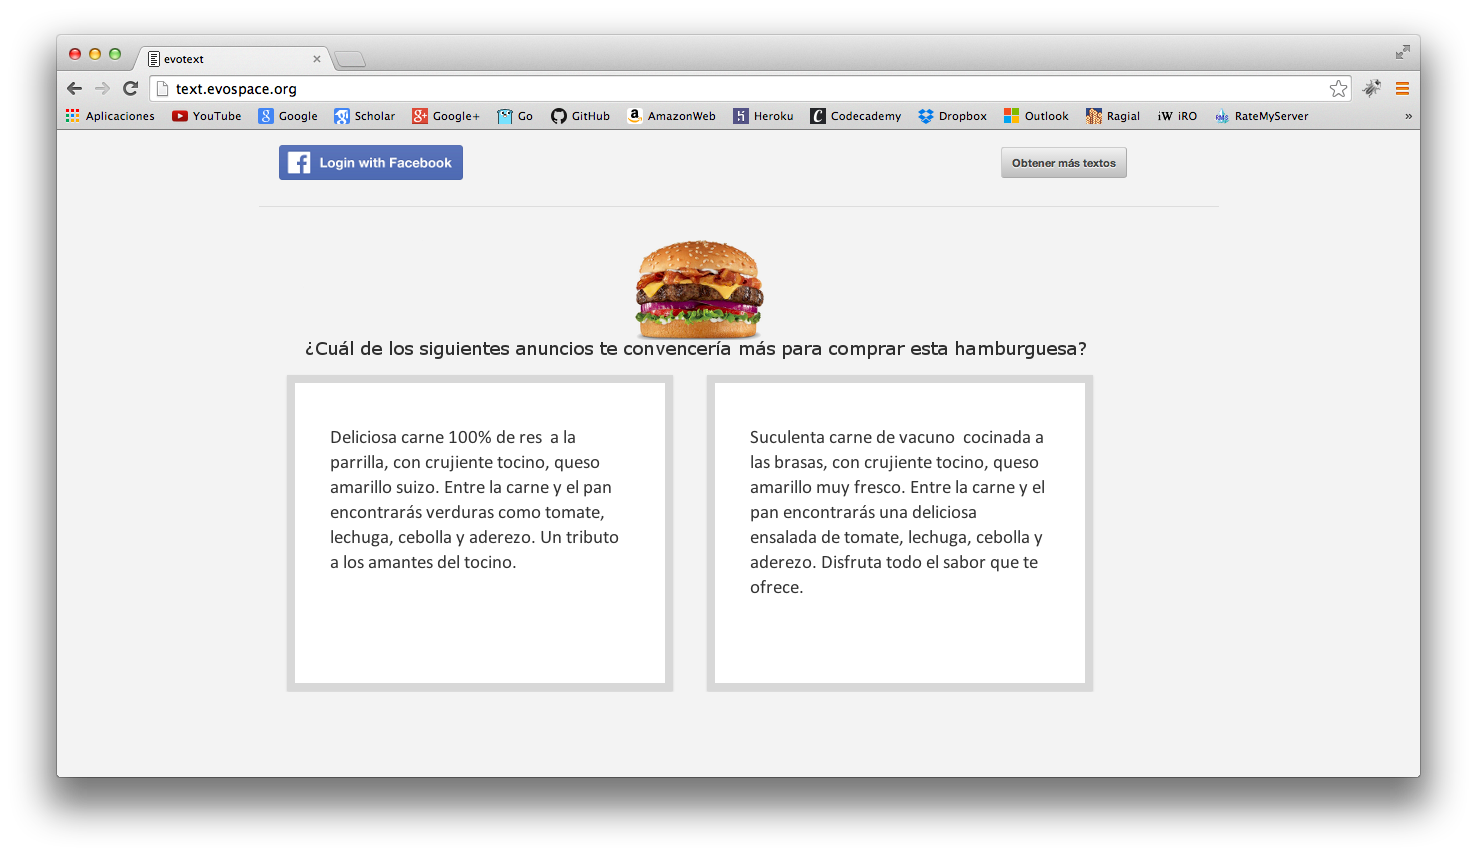
\includegraphics[width=7in]{interfaz.png}} 
  \caption{Interfaz Gráfica} 
\label{interfaz}
\end{figure}

\section{Eficiencia de un Anuncio Publicitario}

La efectividad de un anuncio esta relaciona con la atención que el usuario preste a dicho anuncio, para medir la atención se realizaron 2 pruebas basándonos en el trabajo de Yu-Chen Hsieh y Kuo-Hsiang Chen, 2010. Se realizaron pruebas de reconocimiento y de memoria. Añadimos una prueba para medir la persuasión del anuncio, se les preguntó a los participantes cuál anuncio, entre el generado y el hecho por un experto, creían que era el que más les convencía para comprar el producto que se anunciaba.